%\nonstopmode

\documentclass[11pt]{article}

\usepackage{mathenv}
\usepackage{cancel}
\usepackage{fullpage}
\usepackage{amsmath}
\usepackage{amsfonts}
\usepackage{ulem}
\usepackage{graphicx}
\usepackage{verbatim}
\usepackage{apalike}
\usepackage[usenames, dvipsnames]{color}
\usepackage[colorlinks=true, linkcolor=OliveGreen, citecolor=Purple]{hyperref}

\newcommand{\paperlink}[1]{\href{Documents/papers/#1.pdf}{\cite{#1}}}
\newcommand{\booklink}[2]{\href{Documents/books/#2.pdf}{\cite{#1}}}
\newcommand{\doh}{\partial}
\newcommand{\constant}{\text{ const. }}
\newcommand{\mc}{\mathcal}
\newcommand{\mb}{\mathbb}
\newcommand{\ds}{\displaystyle}
\newcommand{\ts}{\textstyle}

\allowdisplaybreaks

\begin{document}

\title{von Mises orientation maps: notebook}
\author{Carl Smith}
\date{April 27, 2012 - May 11, 2012}
\maketitle
%\tableofcontents

\section*{Notes}
\addcontentsline{toc}{section}{Notes}

\subsection*{Wednesday, June 20, 2012}
Coding up block-wise Gibbs sampling of orientation maps.

\subsection*{Friday, June 8, 2012}
Ran some long HMC samplings overnight and it seems that after a long time the samples do become relatively smooth, though not as smooth as the Gibbs samples after only a few sweeps. (Run $\tt{smoothness}$ in $\tt{hpme/som/matoutfiles/create\_frames\_sampling\_hmc}$ to see results of overnight runs.)

Maybe given that the $q_{ij}$ in this HMC sampling are angular variables, and since we're trying to sample from a very multimodal distribution, we can somehow kick $q_{ij}$'s together so that they go from one basin to another.

\subsection*{Thursday, June 7, 2012}
Liam asked me to compare inference on the low-rank von Mises grid model of orientation maps by Gibbs sampling (element-wise or block-wise) to inference by some other standard method like HMC. So I've coded up both the element-wise Gibbs sampler and an HMC sampler. Gibbs sampling starting from a independently uniform random orientation map, the sample becomes smooth quickly ($\sim10$ sweeps) and pretty much converges on one map. The HMC, on the other hand, starting from random, does not explore state space effectively for the best by-hand selected parameter values (step-size $\epsilon$ and number of steps $L$). Then again, maybe the procedure of Gibbs sampling is itself suspect since it converges to a particular smooth map rather than wandering through the space of smooth maps.

It is mentioned on the web that population Monte Carlo is good for sampling from highly multimodal distributions.

\subsection*{Tuesday, May 1, 2012}
Talked to Liam today. He suggests that I do a quick experiment with synthetic data to show some results on the 2D orientation map at the uptown talk next Monday. In particular I am to 1) generate smooth 2D fields of orientations from the low-rank model using Gibbs sampling on the prior, 2) generate von Mises observations at each location and 3) estimate the orientations given the observations by block-wise Gibbs sampling. I should produce some figure like a colormap or a vector field depicting the orientation over the region.

Another matter is non-grid approaches. How should neurons be connected by these sum-of-separables potentials when they are randomly placed throughout some region?

\subsection*{Monday, April 30, 2012}

Spoke with Kamiar for a while over lunch. In his setup, the observations $Y$ are drawn from a Poisson distribution parametrized by the angle $X$:
%
\begin{align*}
y_t \sim Poiss(a\cos x_t + b\sin x_t).
\end{align*}

\noindent Also, I need to confirm that the block-wise Gibbs sampling approach is valid. Also, Kamiar points me to \paperlink{Macke_2009} for information on the observation distribution.

\subsection*{Saturday, April 28, 2012}

\subsubsection*{A graphical model of pinwheel cells}

Figure \ref{fig:som_gm0} is a graphical model of orientation selectivity in a grid of pinwheel cells. (To ask Kamiar: what topology is the most appropriate?) The following edge potentials serve to smooth the orientation maps, coupling adjacent nodes to keep their values similar:
%
\begin{align*}
p(o_{i,j}|o_{i-1,j}) &\propto \sum_{k=0}^R e^{\kappa \cos\left(o_{i-1,j}-\frac{2\pi k}{R+1}\right)} e^{\kappa \cos\left(o_{i,j}-\frac{2\pi k}{R+1}\right)} \\
p(o_{i,j}|o_{i,j-1}) &\propto \sum_{k=0}^R e^{\kappa \cos\left(o_{i,j-1}-\frac{2\pi k}{R+1}\right)} e^{\kappa \cos\left(o_{i,j}-\frac{2\pi k}{R+1}\right)}
\end{align*}
%
\begin{figure}[h]
\centering
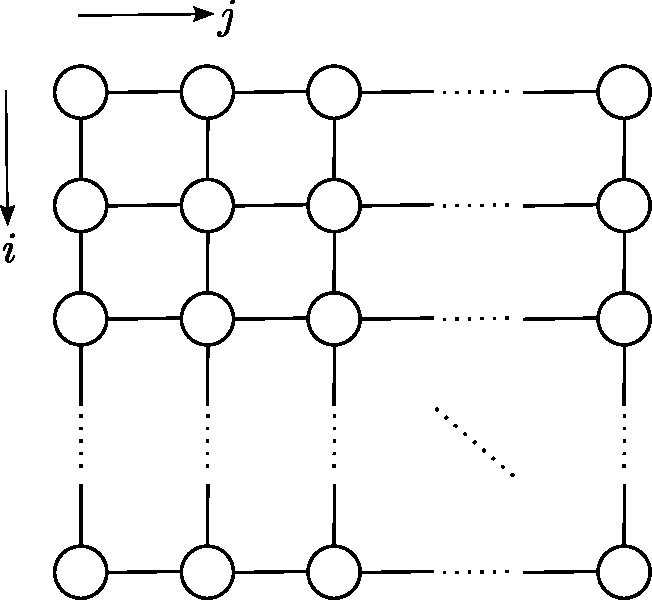
\includegraphics[scale=0.50]{../fig/col_grid_gm}
\caption{A graphical model of orientation selectivity, omitting observed nodes and their dependencies.}
\label{fig:som_gm0}
\end{figure}

\noindent We can suppose that each node has a flat prior $p(o_{i,j})$, as we do here for simplicity, or we can suppose von Mises priors about set modes. (I'm being a bit fast and loose about whether this is a Markov random field or a Bayesian net, dealing with edge potentials as if they were transition probabilities. Hopefully the meaning is clear and I don't think there's anything illogical.) Throughout, the concentration parameter $\kappa$ is assumed to be fixed. With the observations included the graphical model may be depicted as in Figure \ref{fig:som_gm2}, where the small black circles denote the observations which have probability
%
\begin{align*}
p(z_{i,j}|o_{i,j}) &\propto e^{\kappa \cos(z_{i,j}-o_{i,j})}.
\end{align*}

\begin{figure}[h]
\centering
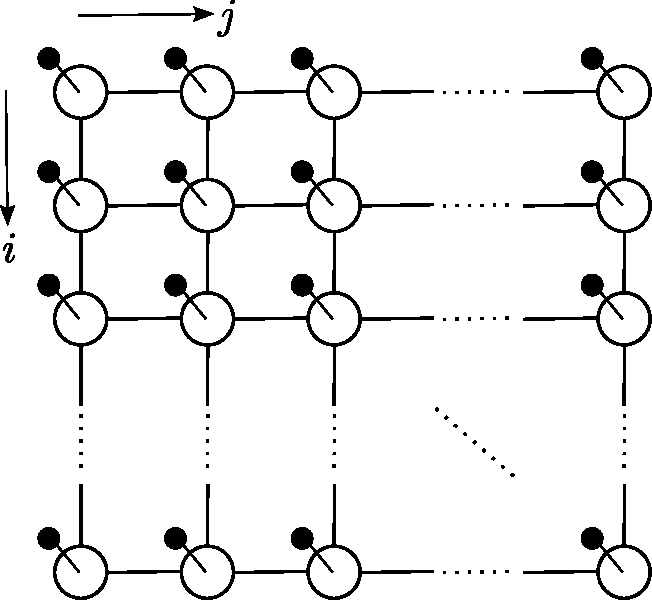
\includegraphics[scale=0.50]{../fig/col_grid_gm_obs}
\caption{A graphical model of orientation selectivity, including observed nodes and their dependencies.}
\label{fig:som_gm2}
\end{figure}

\subsubsection*{The von Mises-Fisher distribution}

On the unit circle, the von Mises distribution can be parametrized by the ``mean" angle $\phi$ where the mode of the density resides:
%
\begin{align*}
f(x|\phi,\kappa) &= \frac{e^{\kappa\cos(x-\phi)}}{2\pi I_0(\kappa)}
\end{align*}

\noindent where $I_0(x)$ is the order 0 modified Bessel function. (Assume throughout that $\kappa$ is fixed.) Instead, however, consider the unit vector $\mathbf{x}$ from the circle's center to the point on the perimeter an angle $x$ away from the $x$-axis. Similarly define $\mathbf{\mu}$ to be the vector with tail at the circle's center and point on the perimeter making the angle $\phi$ with the $x$-axis. This we may write
%
\begin{align*}
f(\mathbf{x}|\mathbf{\mu},\kappa) = \frac{e^{\kappa \mathbf{\mu}^T \mathbf{x}}}{2\pi I_0(\kappa)}.
\end{align*}

\noindent This is more generally an expression for the $p$-dimensional von Mises-Fisher distribution on the surface of the $p$-sphere, where $\mathbf{x}$ and $\mu$ are $p$-vectors and where $(2\pi I_0(\kappa))^{-1}$ is replaced by the more general normalization constant 

\begin{align*}
C_p(\kappa)=\frac{\kappa^{p/2-1}}{(2\pi)^{p/2} I_{p/2-1}(\kappa)}.
\end{align*}

\subsubsection*{The conditional distribution of a column}

Define $\mathbf{r}_k$ to be the unit vector that makes an angle of $\frac{2\pi k}{R+1}$ with the $x$-axis. Define $\mathbf{o}_{i,j}$ to be the vector that makes an angle of $o_{i,j}$ with the $x$-axis. Define $\mathbf{z}_{i,j}$ to be the unit vector that makes an angle of $z_{i,j}$ with the $x$-axis. Suppose that was have marginal estimates for every node and that we wish to block-wise draw a sample from the $j^{th}$ column. Without loss of generality, assume $1<j<N$ where $N$ is the number of columns and $M$ the number of rows. The conditional distribution of the $j^{th}$ column given the rest of the nodes and given the observations is

\begin{align*}
P_j &\equiv p(O_{1:M,j}|O\backslash O_{1:M,j},Z) \\
&= p(O_{1:M,j}|O_{1:M,j-1},O_{1:M,j+1},Z_{1:M,j}) \\
&= p(o_{1,j}|o_{1,j-1},o_{1,j+1},z_{1,j}) \prod_{i=2}^M p(o_{i,j}|o_{i-1,j},o_{i,j-1},o_{i,j+1},z_{i,j}).
\end{align*}

\noindent This first factor is
%
\begin{align*}
p(o_{1,j}|o_{1,j-1},o_{1,j+1},z_{1,j}) &\propto p(o_{1,j-1}) p(o_{1,j}|o_{1,j-1})p(o_{1,j+1}|o_{1,j})p(z_{1,j}|o_{1,j}) \\
&\propto p(o_{1,j}|o_{1,j-1})p(o_{1,j+1}|o_{1,j})p(z_{1,j}|o_{1,j}) \\
&\propto \sum_{k=0}^R e^{\kappa \mathbf{r}_k^T \mathbf{o}_{1,j-1}} e^{\kappa \mathbf{r}_k^T \mathbf{o}_{1,j}}
\sum_{k'=0}^R e^{\kappa \mathbf{r}_{k'}^T \mathbf{o}_{1,j}} e^{\kappa \mathbf{r}_{k'}^T \mathbf{o}_{1,j+1}}
\cdot e^{\kappa \mathbf{z}_{1,j}^T\mathbf{o}_{1,j} }.
\end{align*}

\noindent The second factor is
%
\begin{align*}
p(o_{i,j}|o_{i-1,j},o_{i,j-1},o_{i,j+1},z_{i,j}) &\propto p(o_{i,j-1}) p(o_{i-1,j}) p(o_{i,j}|o_{i,j-1})p(o_{i,j+1}|o_{i,j})p(z_{i,j}|o_{i,j}) \\
&\propto p(o_{i,j}|o_{i,j-1})p(o_{i,j+1}|o_{i,j})p(z_{i,j}|o_{i,j}) \\
&\propto \sum_{k=0}^R e^{\kappa \mathbf{r}_k^T \mathbf{o}_{i,j-1}} e^{\kappa \mathbf{r}_k^T \mathbf{o}_{i,j}}
\sum_{k'=0}^R e^{\kappa \mathbf{r}_{k'}^T \mathbf{o}_{i,j}} e^{\kappa \mathbf{r}_{k'}^T \mathbf{o}_{i,j+1}}
\cdot e^{\kappa \mathbf{z}_{i,j}^T\mathbf{o}_{i,j} }.
\end{align*}

\noindent Putting these together, the conditional distribution is

\begin{align*}
P_j \propto \sum_{k=0}^R &e^{\kappa \mathbf{r}_k^T \mathbf{o}_{1,j-1}} e^{\kappa \mathbf{r}_k^T \mathbf{o}_{1,j}}
\sum_{k'=0}^R e^{\kappa \mathbf{r}_{k'}^T \mathbf{o}_{1,j}} e^{\kappa \mathbf{r}_{k'}^T \mathbf{o}_{1,j+1}}
\cdot e^{\kappa \mathbf{z}_{1,j}^T\mathbf{o}_{1,j} } \times \\
&\prod_{i=2}^T \sum_{k''=0}^R e^{\kappa \mathbf{r}_{k''}^T\mathbf{o}_{i,j-1}} e^{\kappa \mathbf{r}_{k''}^T\mathbf{o}_{i,j}}
\sum_{k'''=0}^R e^{\kappa \mathbf{r}_{k'''}^T\mathbf{o}_{i,j}} e^{\kappa \mathbf{r}_{k'''}^T\mathbf{o}_{i,j+1}}.
\end{align*}

\subsubsection*{Sampling a column block-wise by forward backward}

Along column $j$, starting from the top ($i=1$), we compute forward variables each corresponding to a particular value of the auxiliary value $k_i$ that connects $o_{i,j}$ to $o_{i+1,j}$. It is helpful to have the joint factor graph representation in Figure \ref{fig:som_gm3} in mind.

\begin{align*}
A_1^{(k_1)} &= \int do_{1j} p(o_{1j}) p(k_1|o_{1j}) p(z_{1j}|o_{1j}) \\
&\propto \int do_{1j} \left( \sum_{l_1=0}^R e^{\kappa \mathbf{r}_{l_1}^T \mathbf{o}_{1,j-1}}e^{\kappa \mathbf{r}_{l_1}^T \mathbf{o}_{1j}} \sum_{m_1=0}^R e^{\kappa \mathbf{r}_{m_1}^T \mathbf{o}_{1j}} e^{\kappa \mathbf{r}_{m_1}^T \mathbf{o}_{1,j+1}} \right) e^{\kappa \mathbf{r}_{k_1}^T \mathbf{o}_{1j}} e^{\kappa \mathbf{z}_{1j}^T\mathbf{o}_{1j}} \\
&= \sum_{l_1=0}^R \sum_{m_1=0}^R e^{\kappa (\mathbf{r}_{l_1}^T\mathbf{o}_{1,j-1}+\mathbf{r}_{m_1}^T\mathbf{o}_{1,j+1})} \int do_{1j} e^{\kappa(\mathbf{r}_{l_1}+\mathbf{r}_{m_1}+\mathbf{r}_{k_1}+\mathbf{z}_{1j})^T\mathbf{o}_{1j}} \\
&= \sum_{l_1=0}^R \sum_{m_1=0}^R e^{\kappa (\mathbf{r}_{l_1}^T\mathbf{o}_{1,j-1}+\mathbf{r}_{m_1}^T\mathbf{o}_{1,j+1})} \frac{1}{C_p(\kappa\cdot ||\mathbf{r}_{l_1}+\mathbf{r}_{m_1}+\mathbf{r}_{k_1}+\mathbf{z}_{1j}||)} \\
A_i^{(k_i)} &= \sum_{k_{i-1}=0}^R A_{i-1}^{(k_{i-1})} \int do_{i,j} p(o_{i,j}|k_{i-1})p(k_i|o_{i,j})p(z_{i,j}|o_{i,j}) \\
&\propto \sum_{k_{i-1}=0}^R A_{i-1}^{(k_{i-1})} \int do_{i,j} \left( \sum_{l_i=0}^R e^{\kappa\mathbf{r}_{l_i}^T\mathbf{o}_{i,j-1}} e^{\kappa\mathbf{r}_{l_i}^T\mathbf{o}_{i,j}} \sum_{m_i=0}^R e^{\kappa\mathbf{r}_{m_i}^T\mathbf{o}_{i,j}} e^{\kappa\mathbf{r}_{m_i}^T\mathbf{o}_{i,j+1}}\right) e^{\kappa \mathbf{r}_{k_{i-1}}^T \mathbf{o}_{i,j}} e^{\kappa \mathbf{r}_{k_i}^T \mathbf{o}_{i,j}} \\
&= \sum_{k_{i-1}=0}^R A_{i-1}^{(k_{i-1})} \sum_{l_i=0}^R \sum_{m_i=0}^R e^{\kappa\left(\mathbf{r}_{l_i}^T\mathbf{o}_{i,j-1}+\mathbf{r}_{m_i}^T\mathbf{o}_{i,j+1}\right)} \int do_{i,j} e^{\kappa(\mathbf{r}_{l_i}+\mathbf{r}_{m_i}+\mathbf{r}_{k_{i-1}}+\mathbf{r}_{k_i}+\mathbf{z}_{i,j})^T\mathbf{o}_{i,j}} \\
&= \sum_{k_{i-1}=0}^R A_{i-1}^{(k_{i-1})} \sum_{l_i=0}^R \sum_{m_i=0}^R e^{\kappa\left(\mathbf{r}_{l_i}^T\mathbf{o}_{i,j-1}+\mathbf{r}_{m_i}^T\mathbf{o}_{i,j+1}\right)} \frac{1}{C_p(\kappa\cdot ||\mathbf{r}_{l_i}+\mathbf{r}_{m_i}+\mathbf{r}_{k_{i-1}}+\mathbf{r}_{k_i}+\mathbf{z}_{i,j}||)} 
\end{align*}

\begin{figure}[h]
\centering
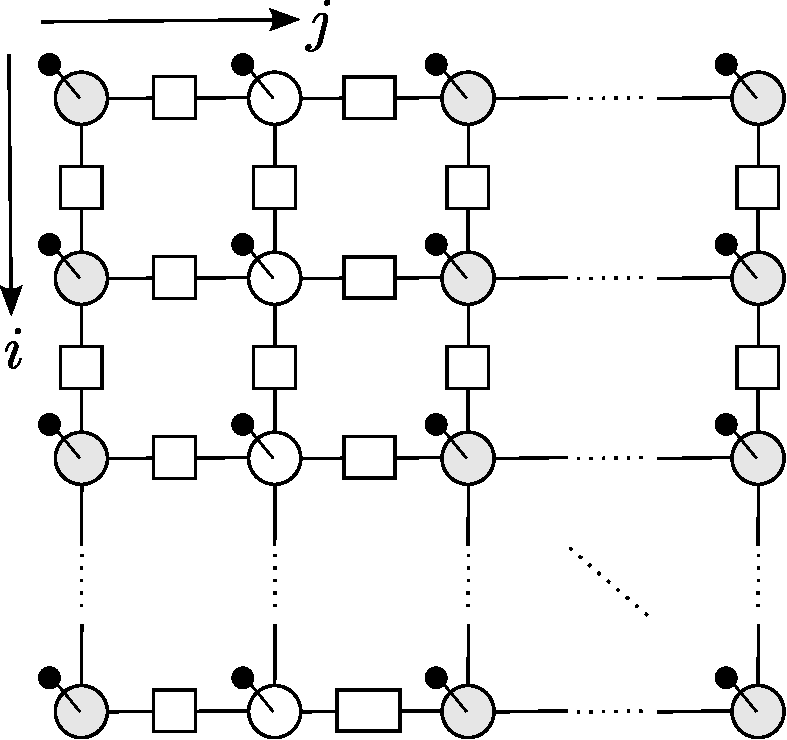
\includegraphics[scale=0.55]{../fig/col_grid_gm_factors}
\caption{A graphical model of orientation selectivity, including observed nodes and auxiliary variables and their dependencies, drawing attention to a forward backward run on the second column from the left. The shaded nodes' values are held as constants, as are the observations. At each step of the forward recursion, to each possible value of $k_i$ corresponds a forward variable $A_i^{(k_i)}$.}
\label{fig:som_gm3}
\end{figure}

\noindent Similarly we may derive backward variables:
%
\begin{align*}
B_M^{(k_{M-1})} &= \int do_{M,j} p(o_{M,j}|k_{M-1,j}) p(z_{M,j}|o_{M,j}) \\
&= \sum_{l_{M}=0}^R \sum_{m_{M}=0}^R 
e^{\kappa\left( \mathbf{r}_{l_{M}}^T \mathbf{o}_{M,j-1}+
\mathbf{r}_{m_{M}}^T \mathbf{o}_{M,j+1}\right)}
\frac{1}{C_p(\kappa\cdot ||\mathbf{r}_{l_{M}}+\mathbf{r}_{m_{M}}+\mathbf{r}_{k_{M-1}}+\mathbf{z}_{M,j}||)} \\
B_i^{k_{i-1}} &= \sum_{k_i=0}^R B_{i+1}^{k_i} \int do_{i,j} p(o_{i,j}|k_{i-1}) p(k_i|o_{i,j}) p(z_{i,j}|o_{i,j}) \\
&= \sum_{k_i=0}^R B_{i+1}^{k_i}
\sum_{l_{i}=0}^R \sum_{m_{i}=0}^R 
e^{\kappa\left( \mathbf{r}_{l_{i}}^T \mathbf{o}_{i,j-1}+
\mathbf{r}_{m_{i}}^T \mathbf{o}_{i,j+1}\right)}
\frac{1}{C_p(\kappa\cdot ||\mathbf{r}_{l_{i}}+\mathbf{r}_{m_{i}}+\mathbf{r}_{k_{i-1}}+\mathbf{r}_{k_{i}}+\mathbf{z}_{i,j}||)}
\end{align*}

\noindent ***DERIVE EXPRESSION FOR SINGLETON MARGINAL IN TERMS OF FORWARD AND BACKWARD VARIABLES.***

\subsection*{Friday, April 27, 2012}
Liam had an idea for using the low-rank models to smooth orientation maps on cortical surface. From an email:

\begin{quotation}
\noindent imagine you observe a bunch of neurons on the cortical surface.  each neuron is labeled by its position on the surface.  we know that in many cases nearby neurons have similar tuning properties.  so if we want to estimate the tuning properties of a bunch of these neurons that we observe simultaneously, it makes sense to share information across neurons by doing some smoothing.  

in V1, for example, the preferred orientation is usually a smooth function of position.  so we might introduce the following simple hierarchical model:

let $o(x,y)$ denote the preferred orientation of the neuron at position $(x,y)$.  we observe some information $z(x,y)$ about each neuron's orientation.  so we can write down
%
\begin{align*}
p(O,Z) &= p(O) p(Z|O) \\
p(Z|O) &= \prod_{x,y} p( z(x,y) | o(x,y) ).
\end{align*}

\noindent now we need a smoothing prior for $p(O)$.  one convenient choice is to use a spatial prior of the low-rank form discussed in \paperlink{Smith_2012}.
%
\begin{align*}
p(O) &= \prod_{x,y} \phi[o(x,y),o(x,y+1)] \phi[o(x,y),o(x+1,y)]
\end{align*}

\noindent here the term $\phi[o(x,y),o(x,y+1)]$ penalizes roughness in the vertical direction, and $\phi[o(x,y),o(x+1,y)]$ penalizes the horizontal direction.

if $\phi(\cdot)$ has the low-rank form discussed in the paper, then inference in this model can proceed via an efficient blockwise gibbs approach: choose a row (or column) of $\{o(x,y)\}_{x=i}$, and draw an exact sample from 
%
\begin{align*}
p( {o(x,y)}_{x=i} | {z(x,y)}_{x=i}, {o(x,y)}_{x=i-1}, {o(x,y)}_{x=i+1} ),
\end{align*}

\noindent using the fast method in \paperlink{Smith_2012}.  iterating across rows and columns gives samples from $P(O|Y)$.
\end{quotation}

Liam has in mind the kind of data described in \paperlink{Ohki_2006}.

\bibliographystyle{apalike}
\bibliography{refs}
\end{document}
